% !TEX root = ../Thesis.tex
\chapter{Mathematical tools}
\section{Power Iterations}
\label{sec:powerIterations}

Power iteration (also called power method) is an iteratively method, 
that approximates biggest eigenvalue of a diagonalizable matrix $A$.

The algorithm starts with a random vector $b_0$ or an approximation of the dominant eigenvector.

\begin{equation}
    \label{eq:powerIterations}
    b_{k+1} = \frac{Ab_k}{||Ab_k||}
\end{equation}

\textbf{TODO:convergence if there is only one largest eigenvalue and if b0 is not orthogonal to the eigenvector associated with the largest eigenvalue.}

The algorithm not necessarily converges. The algorithm will converge, if $A$ has an eigenvalue strictly grater than its other eigenvalues
and the initial vector $b_0$ has a component in direction of an eigenvector, associated with the dominant eigenvector.

\section{Wasserstein metric}
\label{sec:wasserstein-metric}
\textbf{TODO: the difference between Wasserstein and KL divergence for instance is that it is defined (the value is finite) even if the two distributions have not the same support. }


The Wasserstein metric is a distance measure between two probability distributions and it is used in ML as a loss function\cite{learningWithWasserstein}. 
Intuitively, it can can be understood as the minimum cost to transfer the mass of one distribution to the other.
Therefore, it is also known as the \textit{earth mover's distance}.

As \citet{wassersteinGAN} could show, ordinary distance measures like \textit{Total Variation}, \textit{Kullback-Leibler divergence}
and \textit{Jensen-Shannon divergence} are not sensible when learning with distributions supported by manifolds
On the contrary, Wasserstein metric does a good job as loss function in such scenarios.

\section{Radon Transform}
The Radon Transform\cite{radonTransform} is the main mathematically concept of tomographic reconstruction.
It is an integral transformation and the inverse for classical tomography is well defined by the Fourier Transform.

For classical tomography, $R: f \to Rf, f(x,y) \mapsto Rf(\theta, s)$, where $f$ is a 2D image and $x$ and $y$
can be seen as the coordinates within this image. Then, $Rf(f; \theta, s)$ defines a line, where $s$ is the distance 
from the origin and $\theta$ is the angle to the x-axis.

In Figure~\ref{fig:phantom_theta45} and Figure~\ref{fig:phantom_theta45_s14} on can see two plots of different
values for $\theta$ and $s$, where $f(x,y)$ is the Shepp-Logan phantom. The complete $R(\theta=45, s=0)$, 
which is also called \textit{sinogram}, can be see in Figure~\ref{fig:phantom_sinogram}

\begin{figure}[H]
    \centering
    \subbottom[Radon Transform  $R(x;\theta=45, s=0)$\label{fig:phantom_theta45}]{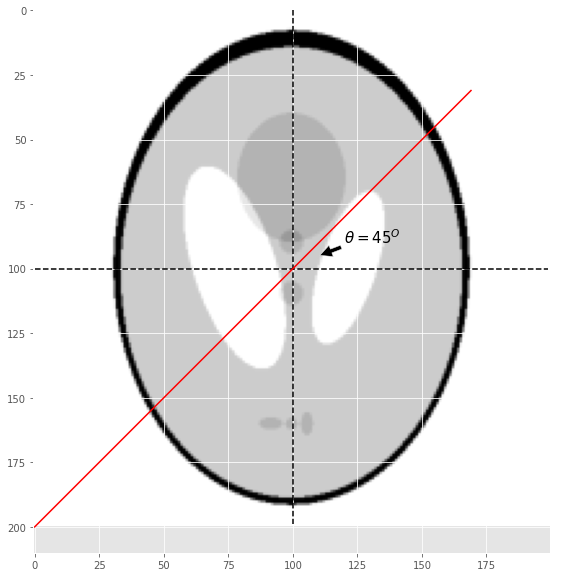
\includegraphics[width=0.3\textwidth]{phantom_theta45.png}}
    \subbottom[Radon Transform  $R(x;\theta=45, s=14.14)$\label{fig:phantom_theta45_s14}]{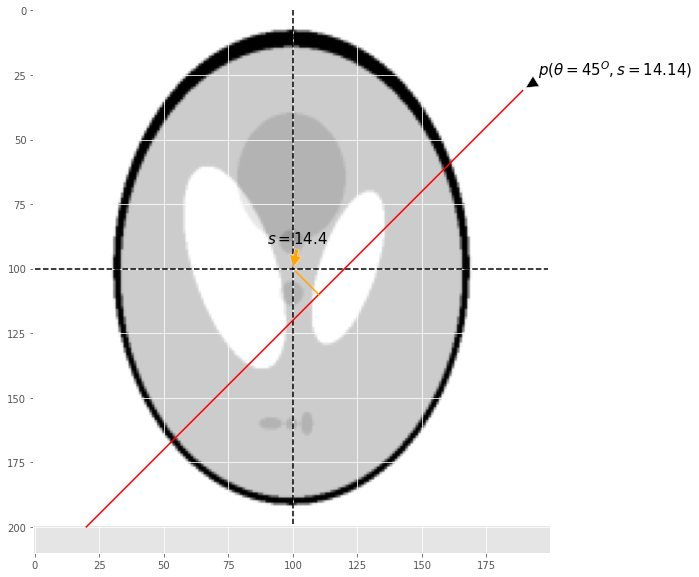
\includegraphics[width=0.3\textwidth]{phantom_theta45_s14.png}}
    \subbottom[Shepp–Logan phantom sinogram of $R(x; \theta=45, s=0)$\label{fig:phantom_sinogram}]{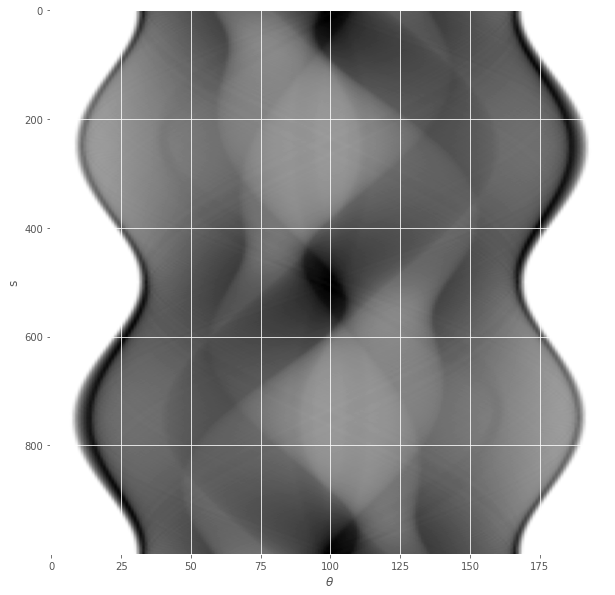
\includegraphics[width=0.3\textwidth]{phantom_sinogram.png}}
    \caption{Examples, where the original object $x$ is the Shepp-Logan phantom.}
\end{figure}